\section{Key Changes}

This section lists key changes made to the RaM process since my dissertation. 

\subsection{Equilibration Step}\label{ss:equilibration}

This change adds a step to the restart of the RaM workflow (Chapter~4, \emph{Restarting Nodal Variables and State Variables}, and step~6 of \emph{Workflow Automation}). The dissertation restarts the simulation directly in dynamics from the remapped fields, with the velocity $\mathbf{v}$ and acceleration $\mathbf{a}$ ``remapped and restarted normally''. A short equilibration step is now taken first. It brings the remapped state back into the dynamic equilibrium it satisfied before the remap, without recording the correction as motion.

\paragraph{Motivation.}
Remapping to a new mesh leaves the restarted state out of discrete equilibrium. Each field is transferred accurately on its own, but the internal forces assembled from the remapped stress on the new mesh no longer balance the remapped inertia and the boundary loads. On a remapped restart of the phase-field plate problem, the nodal fields are recovered exactly: the acceleration at the start of the restart equals its value before the remap, $\sim10^{-8}$. The internal forces, however, imply accelerations of $\sim10^{-3}$, with a maximum of $0.07$. This imbalance is spread over the whole model, including undamaged regions far from the crack, so it is a property of the remap and not of the damage band.

The first time step removes the imbalance by moving the mesh. On this restart the first step moves nodes by up to $2.3\times10^{-3}$, whereas the physical motion over a step of $\Delta t=100$ is only $\|\mathbf{v}\|\Delta t\approx4\times10^{-4}$. The Newmark update (with the HHT-$\alpha$ parameters of Chapter~2) reads this correction as motion:
\begin{equation}
    \mathbf{a}_{n+1} = \frac{1}{\beta\Delta t^2}\left(\mathbf{u}_{n+1}-\mathbf{u}_n\right) - \frac{1}{\beta\Delta t}\mathbf{v}_n - \left(\frac{1}{2\beta}-1\right)\mathbf{a}_n.\label{eq:newmark_accel}
\end{equation}
A fixed correction $\Delta\mathbf{u}$ therefore produces a spurious acceleration of order $\Delta\mathbf{u}/(\beta\Delta t^2)$, which grows as the time step shrinks. The measured maximum first-step acceleration is $5.5\times10^{-7}$ at $\Delta t=100$, $5.3\times10^{-5}$ at $\Delta t=10$, $3.5\times10^{-3}$ at $\Delta t=1$ and $2.9\times10^{-2}$ at $\Delta t=0.1$. A time-step cut after a difficult restart therefore makes the artifact worse rather than better. In TET10 meshes the artifact concentrates on the mid-edge nodes inside the damage band. The ratio of peak mid-edge to corner acceleration there reaches 1.9 on the first restart step, against 1.0 in a continuous run without RaM.

\paragraph{Implementation.}
Before the remap, the state at step $n$ satisfies the HHT-$\alpha$ balance of momentum,
\begin{equation}
    \mathbf{M}\mathbf{a}_n + (1+\alpha)\,\mathbf{f}^\text{int}(\boldsymbol{\sigma}_n) - \alpha\,\mathbf{f}^\text{int}(\boldsymbol{\sigma}_{n-1}) = \mathbf{f}^\text{ext},\label{eq:hht_balance}
\end{equation}
where $\mathbf{f}^\text{int}(\boldsymbol{\sigma}) = \int \boldsymbol{\sigma} : \nabla\mathbf{w}\,dV$ is the internal force of a stress field. The restart now begins with an equilibration step of negligible length ($\Delta t_\text{eq}=10^{-6}$) that solves the same balance on the new mesh for the displacement $\mathbf{u}$, with the inertia and the old stress taken from the remapped fields:
\begin{equation}
    \mathbf{M}\mathbf{a}_\text{rec} + (1+\alpha)\,\mathbf{f}^\text{int}\big(\boldsymbol{\sigma}(\mathbf{u})\big) - \alpha\,\mathbf{f}^\text{int}(\boldsymbol{\sigma}_{n-1,\text{rec}}) = \mathbf{f}^\text{ext}.\label{eq:equilibration}
\end{equation}
If the remap introduced no error, $\mathbf{u}$ does not move and the restart continues exactly as before. Otherwise the step absorbs the remap error into the configuration. One such step is normally enough, after which the time step returns to its dynamic value. During the equilibration window:
\begin{itemize}
    \item The inertial force is \emph{frozen} at the remapped acceleration, $\rho\,\mathbf{a}_\text{rec}$, in place of the Newmark inertia term, so the step keeps the inertial force the body carried before the remap.
    \item The HHT-$\alpha$ terms are carried. The old stress in Eq.~\eqref{eq:equilibration} is the stress of the step before the remap, $\boldsymbol{\sigma}_{n-1}$, which is remapped along with the stress. Like the stress, it is transferred component by component and not through the Lie-group interpolation, since a stress does not belong to a Lie group.
    \item The Newmark velocity and acceleration updates are suspended, so the equilibrating displacement is not recorded as motion. The remapped $\mathbf{v}$ and $\mathbf{a}$ therefore reach the first dynamic step unchanged.
    \item The coupling between the mechanics and the damage problem is held: the damage problem keeps its previous driving energy, and its damage is not passed back to the mechanics.
\end{itemize}
The last point is needed because the phase-field problem is rate independent. Left active, it re-solves against the newly equilibrated mechanics however short the step is, and on test restarts the damage advanced by 0.011--0.018 during a step that takes no physical time. That damage softens the band, and the first dynamic step answers with a large increment, which reappears as the same acceleration artifact. With the driving energy held, the damage problem sees its old driving force and irreversibility keeps $d$ in place. Quantities that set the coefficients of the damage problem itself, such as the coalescence factor $g_c(\bar{\varepsilon}^p)$, are still passed to it.

\paragraph{Results.}
Table~\ref{table:equilibration} shows the effect of the equilibration step on the HEX8 box problem ($\Delta t=0.181$, $\alpha=-0.3$), restarted at $t=18.824$ from two files: the raw output on the same mesh, and the same state remapped to a new mesh. Each restart is compared with a continuous run without RaM over the first five steps after the restart. For the raw output the state is already in equilibrium and the correct equilibration moves nothing, so this case checks that the step leaves an accurate restart unchanged. The remapped case measures how much of the remap error it removes.

\begin{table}[htbp]
    \centering
    \caption{Relative RMS difference of the nodal fields from a continuous run, over the first five steps after the restart of the HEX8 box problem (range over the steps).}\label{table:equilibration}
    \begin{tabular}{llll}
        \toprule
                                        & Raw output, same mesh   & \multicolumn{2}{c}{Remapped} \\
        \cmidrule(lr){2-2}\cmidrule(lr){3-4}
                                        & $a_x$                   & $a_y$         & $v_y$       \\
        \midrule
        Without equilibration           & $1.3$--$2.1\times10^{-4}$ & 12.6--26.3  & 0.39--0.70 \\
        With equilibration              & $1.7$--$2.8\times10^{-4}$ & 3.5--5.8    & 0.33--0.38 \\
        \bottomrule
    \end{tabular}
\end{table}

\FloatBarrier{}

On the raw output, the equilibration step reproduces the continuous run to the same accuracy as a restart without it, and it moves the mesh by only $\sim10^{-8}$. On the remapped output, it reduces the acceleration error in $y$ 3--5 times and roughly halves the velocity error in $y$. The remaining error, about 3\% in the velocity and displacement in $x$ with or without the step, is remap error that an equilibration step cannot remove.

\subsection{Projecting $\Ubar$ instead of $\U$}
Normally, we project $\U$ and reapply the volume averaging. It was found that more accurate results were obtained if we simply transferred $\Ubar$, and skipped the reapplication of the locking correction.

\subsection{Irreversibility enforcement for TET10 elements}

Previously, we were using a penalty method to enforce irreversiblity the phase-field variable when using TET10 elements. A penalty method used because the normal VI solver did not properly enforce irrerversiblity when used in conjuction with the non-positive definite 2nd order Lagrange-shape functions. 

I have swapped to using second order Berstein shape functions for the phase-field variable, which are positive definite. 

\subsection{Change to Neo-Hookean Formulation}\label{ss:cnh_change}

This change replaces the volumetric part of the compressible Neo-Hookean (CNH) energy of Chapter~2 (Section~\emph{Constitutive Choices}, after Borden et al.) with one that resists element inversion. The isochoric part is unchanged.

\paragraph{Motivation.}
Elements that are both heavily damaged and strongly compressed are the ones that invert at RaM restarts, when the remapped state is brought back into equilibrium on the new mesh. The dissertation's volumetric energy offers only a bounded resistance to collapse. Its Kirchhoff pressure tends to the finite value $-K/2$ as $J\to0$, so a compressive load that exceeds it can drive an element to zero volume, and the solve then fails with a negative Jacobian.

\paragraph{Formulation.}
Both models share the isochoric energy of Chapter~2,
\begin{equation}
    W(\bar{\mathbf{C}}) = \frac{1}{2}G\left(\operatorname{tr}\bar{\mathbf{C}}-3\right),\qquad \bar{\mathbf{C}} = J^{-2/3}\mathbf{C},
\end{equation}
written here without plasticity. They differ in the volumetric energy $U(J)$ and therefore in the volumetric Kirchhoff pressure $p = J\,U'(J)$, the volumetric stress being $p\,\mathbf{I}$. The dissertation uses
\begin{equation}
    U_\text{D}(J) = \frac{1}{2}K\left[\frac{1}{2}\left(J^2-1\right)-\ln J\right],\qquad p_\text{D}(J) = \frac{1}{2}K\left(J^2-1\right).\label{eq:cnh_vol_borden}
\end{equation}
The modified model uses the Seth--Hill volumetric energy of order $m=1$ (Garanger et al., Eq.~4),
\begin{equation}
    U_\text{M}(J) = \frac{1}{4}K\left[\left(J-1\right)^2+\left(J^{-1}-1\right)^2\right],\qquad p_\text{M}(J) = \frac{1}{2}K\left(J-J^{-1}\right)\left(J+J^{-1}-1\right).\label{eq:cnh_vol_jay}
\end{equation}
The deviatoric part of the Seth--Hill model in the same reference is not adopted; only the volumetric energy changes.

\paragraph{Comparison.}
Figure~\ref{fig:cnh_potentials} compares the two volumetric responses.
\begin{itemize}
    \item \textbf{Small strain.} Both energies vanish at $J=1$ and have $U''(1)=K$, so the two models have the same bulk modulus and agree for small volume changes.
    \item \textbf{Tension.} For $J\to\infty$ both grow as $U\sim KJ^2/4$ and $p\sim KJ^2/2$, so their responses to large expansion are similar.
    \item \textbf{Compression.} Here they differ. As $J\to0$, $U_\text{D}$ grows only logarithmically and $p_\text{D}\to-K/2$, a bounded pressure. $U_\text{M}$ grows as $K/(4J^2)$ and $p_\text{M}\sim-K/(2J^2)$, which diverges. The modified model therefore resists collapse with a pressure that grows without bound as the element approaches inversion.
    \item \textbf{Symmetry.} $U_\text{M}(J)=U_\text{M}(1/J)$: compressing a volume by a factor costs the same energy as expanding it by that factor. The dissertation's energy is not symmetric and favors compression.
\end{itemize}

% Volumetric energy U(J) and Kirchhoff pressure p(J) = J U'(J) of the two compressible Neo-Hookean
% models, both normalized by the bulk modulus K.
%   Dissertation (Borden et al.):  U = (K/2)[(J^2-1)/2 - ln J],      p = (K/2)(J^2 - 1)
%   Modified (CNHJay):             U = (K/4)[(J-1)^2 + (1/J-1)^2],  p = (K/2)(J - 1/J)(J + 1/J - 1)
\pgfplotsset{
    cnhaxis/.style={
            width=0.9\linewidth,
            height=0.7\linewidth,
            xmin=0.25, xmax=2.5,
            xlabel={$J$},
            grid=major,
            legend cell align=left,
            legend style={font=\scriptsize},
        },
    cnhborden/.style={blue, line width=1.2pt, domain=0.25:2.5, samples=200},
    cnhjay/.style={red, line width=1.2pt, dashed, domain=0.25:2.5, samples=200},
}
\begin{figure}[htbp]
    \centering
    \begin{subfigure}[t]{0.48\textwidth}
        \centering
        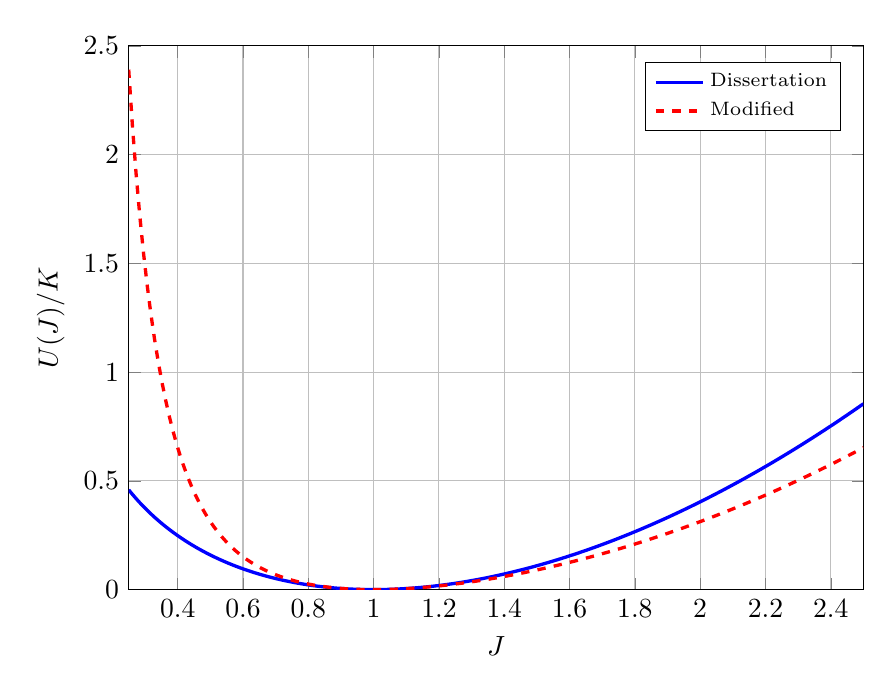
\begin{tikzpicture}
            \begin{axis}[cnhaxis, ymin=0, ymax=2.5, ylabel={$U(J)/K$}, legend pos=north east]
                \addplot[cnhborden] {0.5*(0.5*(x^2-1) - ln(x))};
                \addlegendentry{Dissertation}
                \addplot[cnhjay] {0.25*((x-1)^2 + (1/x-1)^2)};
                \addlegendentry{Modified}
            \end{axis}
        \end{tikzpicture}
        \caption{Volumetric energy}\label{fig:cnh_energy}
    \end{subfigure}
    \hfill
    \begin{subfigure}[t]{0.48\textwidth}
        \centering
        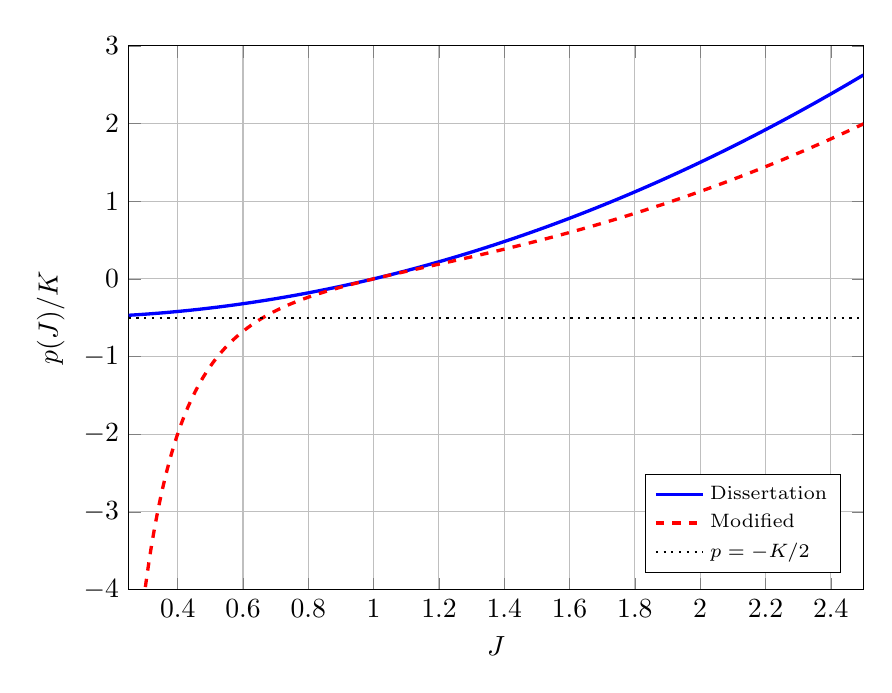
\begin{tikzpicture}
            \begin{axis}[cnhaxis, ymin=-4, ymax=3, ylabel={$p(J)/K$}, legend pos=south east, restrict y to domain=-10:10]
                \addplot[cnhborden] {0.5*(x^2-1)};
                \addlegendentry{Dissertation}
                \addplot[cnhjay] {0.5*(x-1/x)*(x+1/x-1)};
                \addlegendentry{Modified}
                \addplot[black, dotted, line width=0.8pt, domain=0.25:2.5] {-0.5};
                \addlegendentry{$p=-K/2$}
            \end{axis}
        \end{tikzpicture}
        \caption{Volumetric Kirchhoff pressure}\label{fig:cnh_pressure}
    \end{subfigure}
    \caption{Volumetric response of the dissertation's compressible Neo-Hookean model (Eq.~\eqref{eq:cnh_vol_borden}) and the modified model (Eq.~\eqref{eq:cnh_vol_jay}), normalized by the bulk modulus. Both have the same small-strain bulk modulus at $J=1$. As $J\to0$ the dissertation's pressure tends to the finite limit $-K/2$, whereas the modified pressure diverges.}\label{fig:cnh_potentials}
\end{figure}


\paragraph{Consequences for the fracture model.}
The modified model has no volumetric--deviatoric split: the whole energy $U_\text{M}+W$ is active and degraded by $g(d)$, including the compressive volumetric part, which the dissertation's split leaves undegraded. A fully damaged element is therefore also softened in compression. It still resists inversion, because the degraded pressure $g(d)\,p_\text{M}$ diverges as $J\to0$ for any residual stiffness $g(d)\geq\eta>0$, whereas the undegraded $p_\text{D}$ of the split model remains bounded. The return mapping of Borden et al.\ (Chapter~2) uses the same volumetric response $p_\text{M}$, also without an energy split.

\FloatBarrier{}

\subsection{Custom Jacobian Damper}\label{ss:damper}

This change adds a damper to the Newton solve of the mechanics, used on RaM restarts. It limits each Newton step so that no element of the deformed mesh inverts.

\paragraph{Motivation.}
The first Newton iterations of a restart equilibrate the remapped state, which starts out of balance (Section~\ref{ss:equilibration}). On meshes with strongly distorted elements, such as the thin, curved TET10 elements along a damage band, a full Newton step can fold an element: the determinant of its element map becomes negative at a quadrature point, and the residual can no longer be evaluated. This happens however small the time step is, because the step that folds the element is the equilibration of the remapped state and not the load increment. A damper that evaluates each element at the trial configuration cannot handle this case: on a folded element it fails instead of shortening the step.

\paragraph{Formulation.}
The damper never evaluates a trial configuration. For a Newton update $\Delta\mathbf{u}$, the configuration after a fraction $\lambda\in(0,1]$ of the step has nodal positions $\mathbf{x}_a(\lambda) = \mathbf{x}_a + \lambda\,\Delta\mathbf{u}_a$, where $\mathbf{x}_a$ are the current nodal positions. At a quadrature point $\boldsymbol{\xi}_q$ of an element, the Jacobian of the element map is therefore linear in $\lambda$,
\begin{equation}
    \mathbf{J}(\lambda) = \mathbf{J}_0 + \lambda\,\Delta\mathbf{J},\qquad
    \mathbf{J}_0 = \sum_a \mathbf{x}_a \otimes \nabla_{\boldsymbol{\xi}} N_a(\boldsymbol{\xi}_q),\qquad
    \Delta\mathbf{J} = \sum_a \Delta\mathbf{u}_a \otimes \nabla_{\boldsymbol{\xi}} N_a(\boldsymbol{\xi}_q),
\end{equation}
where $N_a$ are the shape functions of the displacement and $\nabla_{\boldsymbol{\xi}}N_a$ their gradients on the master element. Its determinant $\det\mathbf{J}(\lambda)$ is a polynomial in $\lambda$ of degree at most three. Both $\mathbf{J}_0$ and $\Delta\mathbf{J}$ follow from the current configuration and the update alone, so no trial configuration is ever evaluated.

At each quadrature point the damper finds the first step fraction at which the determinant has dropped to a fraction $r_\text{min}$ of its current value,
\begin{equation}
    \lambda^\ast_q = \min\left\{\lambda\in(0,1] : \det\mathbf{J}(\lambda) \leq r_\text{min}\det\mathbf{J}_0\right\},
\end{equation}
by sampling $\lambda$ along the step to bracket the first crossing and refining it by bisection (Figure~\ref{fig:damper_schematic}). Quadrature points whose determinant does not reach the floor within the step impose no limit. The step is then scaled by
\begin{equation}
    \text{damping} = \begin{cases} 1 & \text{if } \lambda^\ast \geq 1, \\ s\,\lambda^\ast & \text{otherwise}, \end{cases}
    \qquad \lambda^\ast = \min_{\text{elements},\,q}\lambda^\ast_q,
\end{equation}
with a safety factor $s<1$. A Newton step that does not approach an inversion is taken in full, so the damper does not slow the convergence of a regular solve. If an element is already inverted at the current configuration, the step is reduced to $10^{-3}$ so that the solve can creep out of it.

% Schematic of the step limit: the Jacobian determinant at one quadrature point along the Newton
% step, det(J0 - lambda dJ), a polynomial in lambda. The curve is illustrative, not simulation data.
\begin{figure}[htbp]
    \centering
    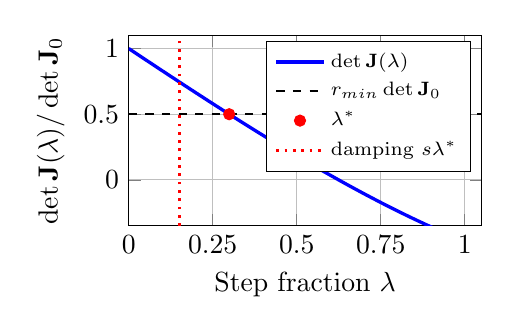
\begin{tikzpicture}
        \begin{axis}[
                width=0.5\linewidth,
                height=0.33\linewidth,
                xmin=0, xmax=1.05,
                ymin=-0.35, ymax=1.1,
                xlabel={Step fraction $\lambda$},
                ylabel={$\det\mathbf{J}(\lambda)/\det\mathbf{J}_0$},
                xtick={0,0.25,0.5,0.75,1},
                legend pos=north east,
                legend cell align=left,
                legend style={font=\scriptsize},
                grid=major,
            ]
            \addplot[blue, line width=1.2pt, domain=0:1, samples=200] {(1-1.6*x)*(1-0.4*x)*(1+0.3*x)};
            \addlegendentry{$\det\mathbf{J}(\lambda)$}
            \addplot[black, dashed, line width=0.8pt, domain=0:1.05] {0.5};
            \addlegendentry{$r_\text{min}\det\mathbf{J}_0$}
            \addplot[red, only marks, mark=*, mark size=2pt] coordinates {(0.299,0.5)};
            \addlegendentry{$\lambda^\ast$}
            \addplot[red, dotted, line width=1pt] coordinates {(0.15,-0.35) (0.15,1.1)};
            \addlegendentry{damping $s\lambda^\ast$}
        \end{axis}
    \end{tikzpicture}
    \caption{Schematic of the step limit at one quadrature point. The determinant of the element map is a polynomial in the step fraction $\lambda$. The damper finds the first $\lambda^\ast$ at which it drops to $r_\text{min}$ times its current value, and the Newton step is scaled to $s\lambda^\ast$ (here $s=r_\text{min}=0.5$; the curve is illustrative).}\label{fig:damper_schematic}
\end{figure}


\paragraph{Use.}
The determinant is checked only at the quadrature points, so an element can still fold between them. Conservative settings guard against that: $s = 0.5$ and $r_\text{min} = 0.5$ were needed on the restarts of the TET10 fracture problem. The step must also be limited before the residual is evaluated at it, so a backtracking line search, which evaluates the residual at the full step first, cannot be used with the damper.

\FloatBarrier{}